\documentclass{beamer}
\usetheme{ConnectivityLab}
\usepackage{times}
\usepackage{graphicx}
\usepackage{verbatim}
\usepackage{outlines}
\usepackage{fancyhdr}
\usepackage{subfigure}
\usepackage{cancel}
\usepackage{bibentry}
\usepackage{varwidth}
\usepackage{etoolbox}
\usepackage{epstopdf}

%%%%%%%%%%%%%%%%%%%%%%%%%%%%%%%%%%%%%%%%%%%%%%%%%%%%%%
%%%%%%%%%%%%%%%%%%%%%%%%%%%%%%%%%%%%%%%%%%%%%%%%%%%%%%

\title {
    Progress Report
}
\author {
    Yin-Hong Hsu
}
\date {
    03 30, 2018
}

%%%%%%%%%%%%%%%%%%%%%%%%%%%%%%%%%%%%%%%%%%%%%%%%%%%%%%
%%%%%%%%%%%%%%%%%%%%%%%%%%%%%%%%%%%%%%%%%%%%%%%%%%%%%%

\begin{document}
\begin{frame}
    \titlepage
\end{frame}

%%%%%%%%%%%%%%%%%%%%%%%%%%%%%%%%%%%%%%%%%%%%%%%%%%%%%%
%%%%%%%%%%%%%%%%%%%%%%%%%%%%%%%%%%%%%%%%%%%%%%%%%%%%%%

\begin{frame}{Outline}
    \tableofcontentsgather
    \tableofcontents
\end{frame}

%%%%%%%%%%%%%%%%%%%%%%%%%%%%%%%%%%%%%%%%%%%%%%%%%%%%%%
%%%%%%%%%%%%%%%%%%%%%%%%%%%%%%%%%%%%%%%%%%%%%%%%%%%%%%
\section{Attack model}
\begin{frame}{Attack model}
    \begin{itemize}
        \item {Eavesdropping:}
        \begin{itemize}
            \item[-] the adversary can eavesdrop get unsafe channels to get messages. In the region-based MCS, the sensed information and the corresponding ring signatures are sent through the Internet without encryption so the adversary can get all of them
        \end{itemize}
        \item {Replay attack:}
        \begin{itemize}
            \item[-] after eavesdropping, the adversary can send a copy without modification to AS. In the RCRS, we have added a timestamp in the message structure to prevent this kind of attack so that the overdue messages would be abandoned
        \end{itemize}
    \end{itemize}
\end{frame}
\begin{frame}{Attack model}
    \begin{itemize}
        \item {Brute force:}
        \begin{itemize}
            \item[-] the adversary is able to try every possible keys and try to make the same signature as the one that matches the eavesdropped message. In the 256-bit RCRS scheme, the key space of MU’s private key contains 2 256 possible keys. It is impossible to discover the MU’s private key of the message without extremely powerful computing power
        \end{itemize}
        \item {Intersection attack:}
        \begin{itemize}
            \item[-] If a specific signer changes the ring to use every time, the adversary can easily to find out what public key the signer is actually used
        \end{itemize}
    \end{itemize}
\end{frame}
\begin{frame}{Attack model}
    \begin{itemize}
        \item {Location forgery:}
        \begin{itemize}
            \item[-] In RCRS, if the MU was compromised by adversary, the adversary can tell KA that MU is leaving to another location. So that can remove MU from current ring.
        \end{itemize}
        \item {Fake Base Station:}
        \begin{itemize}
            \item[-] The adversary can use a fake base station to make MU to connect to, and log all traffic includes MU's privacy info. In proposed framework, the SU in Fog Node can provide privacy preserve service.
        \end{itemize}
    \end{itemize}
\end{frame}
\begin{frame}{}
    \begin{figure}[t]
        \centering
        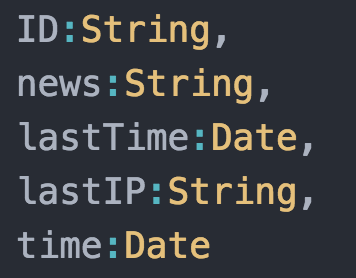
\includegraphics[width=1.0\textwidth]{figures/1.png}
        \setbeamerfont{caption}{size=\tiny}
        \caption{Architecture}
    \end{figure}
\end{frame}
\section{Assumption}
\begin{frame}{Assumption}
    \begin{itemize}
        \item {Fog Nodes are fully trusted}
        \item {Key Authority is maintained by a trusted third party}
        \item {Each Fog Node is a part of an eNB, and the Fog Node can access all parameter in Telecom network}
        \item {The connect between Fog Node to KA and Fog Node to Fog Node is trusted}
    \end{itemize}
\end{frame}
\section{Other benefits}
\begin{frame}{Other benefits}
    \begin{itemize}
        \item {When MU move to another region, MU do not have had to notify KA where it goes, Fog nodes will deal it}
        \item {MU only need to communicate with KA once (register)}
        \item {KA will distribute ring to each region periodic. In RCRS, KA have to broadcast to each MU, AS; In proposed framework, KA only have to send new rings to Fog Nodes, then each Fog Node will distribute the ring to MUs in this region}
    \end{itemize}
\end{frame}
%%%%%%%%%%%%%%%%%%%%%%%%%%%%%%%%%%%%%%%%%%%%%%%%%%%%%%
%%%%%%%%%%%%%%%%%%%%%%%%%%%%%%%%%%%%%%%%%%%%%%%%%%%%%%

\section{References}
\calcreferencespagetotal % Calc your References Page total number
\begin{frame}[allowframebreaks]{References}
    \fontsize{9pt}{13}\selectfont
    \bibliographystyle{IEEEtran}
    \bibliography{IEEEabrv,Citation}
\end{frame}

%%%%%%%%%%%%%%%%%%%%%%%%%%%%%%%%%%%%%%%%%%%%%%%%%%%%%%
%%%%%%%%%%%%%%%%%%%%%%%%%%%%%%%%%%%%%%%%%%%%%%%%%%%%%%
\section{}

\begin{frame}
    \centering
    \Large{Thanks for Your Attentions}
\end{frame}

\end{document}
